\chapter{Mission: Plant}

\emph{\emph{Plant} is a RECON+ mission in which the alliances attempt
  to destroy the campus physical plant using explosives and targets
  chosen to incriminate the opposing side, while not being implicated
  themselves.}

\section{Play Area}
\vspace{-2\parskip}
\noindent\begin{stdminipage}{\linewidth-(2in+1.5em)}
\vspace{0pt}   
\noindent
Whichever player takes Deployment in the Initiative Roll chooses a
corner of the play area for their Deployment Zone, comprised of the
triangle extending 12'' from that corner along the short edge of the
play area and 18'' along the long edge.  The other player takes the
diagonally opposite corner as their Deployment Zone, comprised of a
matching triangle.

The centerline of the play area for purposes of Infiltration and other
rules is the diagonal line between the other two corners.

A Network Terminal is placed at the center of the play area.

\section{Mission Rules}
As part of their deployment, both players secretly choose and record
three scenery pieces entirely within their opponent's half of the play
area as Vulnerable Infrastructure.  Each piece must have a footprint
of at least~4 square inches (e.g., a 2''x2'' square or~2.5'' circle).

\end{stdminipage}
\hfill
\begin{minipage}[t]{2in}\centering
\vspace{4pt}   
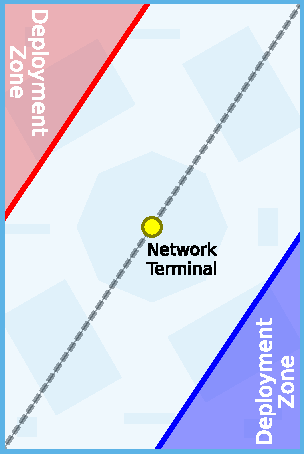
\includegraphics{maps/map-plant}
\end{minipage}

Each player additionally chooses as part of their deployment three of
their models in play (i.e., not markers, troopers in Hidden
Deployment, etc.) to be armed with Bombs (including their Reserve if
they wish).  This is public information revealed following both
players' deployments.

\section{Scoring}

Players may score up to~10 objective points via the following
conditions at game end:
\begin{squishitemize}
%\item 1pt for each of your chosen Vulnerable Infrastructure pieces
%  with a Bomb placed on it at any point.

\item 2pts for each of your chosen Vulnerable Infrastructure pieces
  with a Bomb placed on it.

%\item 1pt if you have more Bombs placed than your opponent.

\item 1pts if there are no enemy Bombs in your table half.

\item 2pt if your Special Agent is in base contact with a Vulnerable
  Infrastructure piece you chose.
  
\item 1pt if more points of the opposing army list have been destroyed.
\end{squishitemize}

\vfill
\clearpage

{\setlength\fboxrule{2pt}
\cfbox{Black}{\begin{minipage}{6.5in}
  \colorbox{Black}{\parbox{\linewidth-2\fboxsep}{\textcolor{White}{\textbf{\large Bomb} \hfill Equipment}}}\\
  \colorbox{White}{\parbox{\linewidth-2\fboxsep}{Deployable, Disposable (2)}}

%  \medskip
%  \textsc{Requirements}
%  \begin{squishitemize}
%  \item A model cannot ever be equipped with more than one Datacube,
%    unless it also possesses Baggage equipment, in which case it may
%    equip two.
%  \end{squishitemize}
  
  \colorbox{Gray!24}{\begin{minipage}{\linewidth-2\fboxsep}

      \medskip
      \textsc{Effects}
      \begin{squishitemize}
      \item A Bomb may be deployed solely by the Place Bomb skill.

      \item A Bomb placed as a Camouflage marker may be Discovered,
        upon which it is replaced by a Bomb marker.  Bombs placed in
        camouflage and then revealed receive the benefit of the CH:
        Mimetism Special Skill; Bombs placed openly do not.

      \item Bombs may only be targeted by the Defuse Bomb skill.  They
        otherwise count as a mission element, the inadvertent
        destruction of which concedes the mission.

      \item Placed Bombs count for scoring purposes whether they are
        camouflaged or not.
        
      \item Bombs have the following profile:

        \smallskip
\hfill\cfbox{Dandelion}{\begin{minipage}{1.85in}\centering
            \colorbox{Dandelion}{\parbox{\linewidth-2\fboxsep}{\textbf{\textcolor{White}{Bomb}}}}

            \noindent\colorbox{Gray!24}{\begin{minipage}{\linewidth-2\fboxsep}\centering

                \medskip
                \noindent\hfill\begin{tabular}[t]{cccc}
                                 \rowcolor{Black} \textbf{\textcolor{White}{ARM}} & \textbf{\textcolor{White}{BTS}} & \textbf{\textcolor{White}{STR}} & \textbf{\textcolor{White}{S}}\\
                                 \hline
                                 0 & 0 & 1 & 1\\
                               \end{tabular}
                             \end{minipage}}
                         \end{minipage}}\hfill\hbox to 0pt{}

        
      \end{squishitemize}
  \end{minipage}}
\end{minipage}}}

{\setlength\fboxrule{2pt}
\cfbox{LimeGreen}{\begin{minipage}{6.5in}
  \colorbox{LimeGreen}{\parbox{\linewidth-2\fboxsep}{\textcolor{White}{\textbf{\large Place Bomb} \hfill Short Skill, ARO, Entire Order}}}\\
  \colorbox{SkyBlue}{\parbox{\linewidth-2\fboxsep}{\textcolor{White}{Attack}}}

  \medskip
  \textsc{Requirements}
  \begin{squishitemize}
  \item The user must be equipped with one or more Bombs.
  \end{squishitemize}

  \medskip
  \colorbox{Gray!24}{\begin{minipage}{\linewidth-2\fboxsep}

      \medskip
      \textsc{Effects}
      \begin{squishitemize}
      \item The user places a Bomb marker in the play area.

      \item By declaring this skill as an Entire Order, the user may
        instead place a Camouflage marker representing a Bomb.  If an
        enemy model or marker is in the user's Zone of Control and has
        Line of Fire to it then they must pass a Normal WIP roll to do
        so.

      \item The marker must be placed on top or in base contact with
        one of the player's chosen pieces of Vulnerable
        Infrastructure, as well as in base contact with the user or,
        in its Active Turn, any part of its route if it moved.
      \end{squishitemize}
  \end{minipage}}
\end{minipage}}}

{\setlength\fboxrule{2pt}
\cfbox{BrickRed}{\begin{minipage}{6.5in}
  \colorbox{BrickRed}{\parbox{\linewidth-2\fboxsep}{\textcolor{White}{\textbf{\large Defuse Bomb} \hfill Entire Order}}}\\
  \colorbox{SkyBlue}{\parbox{\linewidth-2\fboxsep}{\textcolor{White}{Attack}}}

  \medskip
  \textsc{Requirements}
  \begin{squishitemize}
  \item The user must be a model (not a marker) in base contact with a
    Bomb marker.
  \end{squishitemize}

  \medskip
  \colorbox{Gray!24}{\begin{minipage}{\linewidth-2\fboxsep}

      \medskip
      \textsc{Effects}
      \begin{squishitemize}
      % \item If an enemy model or marker is within the
      %   user's Zone of Control and has Line of Fire to the user then
      %   the latter must pass a Normal WIP roll to do so.

      \item The user takes a Normal WIP roll to attempt defusing the
        Bomb.  Specialist Troops may make two Normal WIP Rolls with
        a~+3 MOD.

      \item If successful the Bomb marker is removed from play.
      \end{squishitemize}
  \end{minipage}}
\end{minipage}}}


\vfill
\vbox to 0pt{}